% ==========================================================================
% INFO 4617 Web Data Science -- Week 14: Automating Data Collection (Chapter 14)
% Build:  TEXINPUTS=../common: BIBINPUTS=../common: latexmk -pdf slides.tex
% (or run `make` from the slides/ directory)
% ==========================================================================
\documentclass[9pt,aspectratio=169]{beamer}
% ==========================================================================
% Shared preamble for INFO 4617 Web Data Science weekly lecture decks
% Based on the Gotham beamer theme (vendored in this directory).
% Each week's slides.tex does:  % ==========================================================================
% Shared preamble for INFO 4617 Web Data Science weekly lecture decks
% Based on the Gotham beamer theme (vendored in this directory).
% Each week's slides.tex does:  % ==========================================================================
% Shared preamble for INFO 4617 Web Data Science weekly lecture decks
% Based on the Gotham beamer theme (vendored in this directory).
% Each week's slides.tex does:  \input{preamble}  (with common/ on TEXINPUTS)
% then sets \title/\subtitle/\author/\date and \begin{document}.
% ==========================================================================

\usetheme{gotham}

\usepackage{fbb}
\usepackage{booktabs}
\usepackage{graphicx}
\usepackage{tikz}
\usepackage{xcolor}
\usepackage{multirow}
\usepackage{listings}
\usetikzlibrary{positioning, arrows.meta, shapes}

% Bibliography
\usepackage[style=authoryear,
            backend=biber,
            maxcitenames=1,
            uniquename=false,
            uniquelist=false]{biblatex}
\addbibresource{bibliography.bib}

\gothamset{sectiontocframe default=off}

% ------------------------------------------------------------------ colors
\definecolor{cugold}{HTML}{CFB87C}
\definecolor{tab-red}{HTML}{E15759}
\definecolor{tab-orange}{HTML}{F28E2B}
\definecolor{tab-blue}{HTML}{4E79A7}
\definecolor{tab-cyan}{HTML}{76B7B2}
\definecolor{tab-green}{HTML}{59A14F}
\definecolor{tab-yellow}{HTML}{EDC948}
\definecolor{tab-purple}{HTML}{B07AA1}
\definecolor{tab-pink}{HTML}{FF9DA7}
\definecolor{tab-brown}{HTML}{9C755F}
\definecolor{tab-gray}{HTML}{BAB0AC}

\setbeamercolor{frametitle}{fg=black, bg=cugold}
\setbeamercolor{progress bar}{fg=cugold, bg=cugold!20}

\setbeamercolor{block title alerted}{fg=black, bg=cugold}
\setbeamercolor{block body alerted}{fg=black, bg=cugold!10}

% ------------------------------------------------------------------ footline
\setbeamertemplate{footline}{
  \begin{beamercolorbox}[wd=\paperwidth,ht=2.5ex,dp=1ex,right]{footline}
    {\footnotesize \insertframenumber{} of \inserttotalframenumber}
    \hspace*{2ex}
  \end{beamercolorbox}
}

% ------------------------------------------------------------------ helpers
\newcommand{\bottomcite}[1]{
    \vspace*{\fill}
    \vspace{-\baselineskip}
    {\tiny
    \rule{\textwidth}{0.3pt}\\
    #1
    }
    \vspace{0.5ex}
}

% Consistent code styling for the Wednesday "applied notebook" frames.
\lstdefinestyle{wds}{
    basicstyle=\ttfamily\scriptsize,
    keywordstyle=\color{tab-blue}\bfseries,
    commentstyle=\color{tab-green},
    stringstyle=\color{tab-orange},
    showstringspaces=false,
    breaklines=true,
    columns=fullflexible,
    language=Python,
    aboveskip=0.4em,
    belowskip=0.4em,
}
\lstset{style=wds}

% \dayband{Day}{Topic} -- a lightweight section divider label used to mark
% Monday / Wednesday / Friday within a week's deck.
\newcommand{\dayband}[2]{{\large\textbf{#1}}\;\textcolor{tab-gray}{\textbar}\;#2}
  (with common/ on TEXINPUTS)
% then sets \title/\subtitle/\author/\date and \begin{document}.
% ==========================================================================

\usetheme{gotham}

\usepackage{fbb}
\usepackage{booktabs}
\usepackage{graphicx}
\usepackage{tikz}
\usepackage{xcolor}
\usepackage{multirow}
\usepackage{listings}
\usetikzlibrary{positioning, arrows.meta, shapes}

% Bibliography
\usepackage[style=authoryear,
            backend=biber,
            maxcitenames=1,
            uniquename=false,
            uniquelist=false]{biblatex}
\addbibresource{bibliography.bib}

\gothamset{sectiontocframe default=off}

% ------------------------------------------------------------------ colors
\definecolor{cugold}{HTML}{CFB87C}
\definecolor{tab-red}{HTML}{E15759}
\definecolor{tab-orange}{HTML}{F28E2B}
\definecolor{tab-blue}{HTML}{4E79A7}
\definecolor{tab-cyan}{HTML}{76B7B2}
\definecolor{tab-green}{HTML}{59A14F}
\definecolor{tab-yellow}{HTML}{EDC948}
\definecolor{tab-purple}{HTML}{B07AA1}
\definecolor{tab-pink}{HTML}{FF9DA7}
\definecolor{tab-brown}{HTML}{9C755F}
\definecolor{tab-gray}{HTML}{BAB0AC}

\setbeamercolor{frametitle}{fg=black, bg=cugold}
\setbeamercolor{progress bar}{fg=cugold, bg=cugold!20}

\setbeamercolor{block title alerted}{fg=black, bg=cugold}
\setbeamercolor{block body alerted}{fg=black, bg=cugold!10}

% ------------------------------------------------------------------ footline
\setbeamertemplate{footline}{
  \begin{beamercolorbox}[wd=\paperwidth,ht=2.5ex,dp=1ex,right]{footline}
    {\footnotesize \insertframenumber{} of \inserttotalframenumber}
    \hspace*{2ex}
  \end{beamercolorbox}
}

% ------------------------------------------------------------------ helpers
\newcommand{\bottomcite}[1]{
    \vspace*{\fill}
    \vspace{-\baselineskip}
    {\tiny
    \rule{\textwidth}{0.3pt}\\
    #1
    }
    \vspace{0.5ex}
}

% Consistent code styling for the Wednesday "applied notebook" frames.
\lstdefinestyle{wds}{
    basicstyle=\ttfamily\scriptsize,
    keywordstyle=\color{tab-blue}\bfseries,
    commentstyle=\color{tab-green},
    stringstyle=\color{tab-orange},
    showstringspaces=false,
    breaklines=true,
    columns=fullflexible,
    language=Python,
    aboveskip=0.4em,
    belowskip=0.4em,
}
\lstset{style=wds}

% \dayband{Day}{Topic} -- a lightweight section divider label used to mark
% Monday / Wednesday / Friday within a week's deck.
\newcommand{\dayband}[2]{{\large\textbf{#1}}\;\textcolor{tab-gray}{\textbar}\;#2}
  (with common/ on TEXINPUTS)
% then sets \title/\subtitle/\author/\date and \begin{document}.
% ==========================================================================

\usetheme{gotham}

\usepackage{fbb}
\usepackage{booktabs}
\usepackage{graphicx}
\usepackage{tikz}
\usepackage{xcolor}
\usepackage{multirow}
\usepackage{listings}
\usetikzlibrary{positioning, arrows.meta, shapes}

% Bibliography
\usepackage[style=authoryear,
            backend=biber,
            maxcitenames=1,
            uniquename=false,
            uniquelist=false]{biblatex}
\addbibresource{bibliography.bib}

\gothamset{sectiontocframe default=off}

% ------------------------------------------------------------------ colors
\definecolor{cugold}{HTML}{CFB87C}
\definecolor{tab-red}{HTML}{E15759}
\definecolor{tab-orange}{HTML}{F28E2B}
\definecolor{tab-blue}{HTML}{4E79A7}
\definecolor{tab-cyan}{HTML}{76B7B2}
\definecolor{tab-green}{HTML}{59A14F}
\definecolor{tab-yellow}{HTML}{EDC948}
\definecolor{tab-purple}{HTML}{B07AA1}
\definecolor{tab-pink}{HTML}{FF9DA7}
\definecolor{tab-brown}{HTML}{9C755F}
\definecolor{tab-gray}{HTML}{BAB0AC}

\setbeamercolor{frametitle}{fg=black, bg=cugold}
\setbeamercolor{progress bar}{fg=cugold, bg=cugold!20}

\setbeamercolor{block title alerted}{fg=black, bg=cugold}
\setbeamercolor{block body alerted}{fg=black, bg=cugold!10}

% ------------------------------------------------------------------ footline
\setbeamertemplate{footline}{
  \begin{beamercolorbox}[wd=\paperwidth,ht=2.5ex,dp=1ex,right]{footline}
    {\footnotesize \insertframenumber{} of \inserttotalframenumber}
    \hspace*{2ex}
  \end{beamercolorbox}
}

% ------------------------------------------------------------------ helpers
\newcommand{\bottomcite}[1]{
    \vspace*{\fill}
    \vspace{-\baselineskip}
    {\tiny
    \rule{\textwidth}{0.3pt}\\
    #1
    }
    \vspace{0.5ex}
}

% Consistent code styling for the Wednesday "applied notebook" frames.
\lstdefinestyle{wds}{
    basicstyle=\ttfamily\scriptsize,
    keywordstyle=\color{tab-blue}\bfseries,
    commentstyle=\color{tab-green},
    stringstyle=\color{tab-orange},
    showstringspaces=false,
    breaklines=true,
    columns=fullflexible,
    language=Python,
    aboveskip=0.4em,
    belowskip=0.4em,
}
\lstset{style=wds}

% \dayband{Day}{Topic} -- a lightweight section divider label used to mark
% Monday / Wednesday / Friday within a week's deck.
\newcommand{\dayband}[2]{{\large\textbf{#1}}\;\textcolor{tab-gray}{\textbar}\;#2}


\title[Week 14 · Automation]{{\Huge Automating Data Collection}}
\subtitle{Week 14 · Practice module · Textbook Chapter 14}
\author[Keegan]{\textbf{Brian C. Keegan, Ph.D.} \\ Associate Professor, Department of Information Science \\ University of Colorado Boulder}
\date{November 16, 18 \& 20, 2026}

\begin{document}

\maketitle

% -------------------------------------------------------------------------
\begin{frame}{This week at a glance}
    \begin{columns}[T]
        \begin{column}{0.62\textwidth}
            We move scraping off your laptop and into the cloud --- code that collects data on a schedule, unattended.

            \vspace{1em}

            \dayband{Monday}{Concepts \& notebook intro}
            \begin{itemize}\small
                \item From exploration to production; why a time series beats a snapshot
            \end{itemize}

            \vspace{0.5em}

            \dayband{Wednesday}{Notebook lab}
            \begin{itemize}\small
                \item Notebook $\rightarrow$ script $\rightarrow$ GitHub Actions: schedule it, monitor it, harden it
            \end{itemize}

            \vspace{0.5em}

            \dayband{Friday}{Textbook revisions}
            \begin{itemize}\small
                \item Propose \& peer-review pull requests improving Chapter 14
            \end{itemize}
        \end{column}
        \begin{column}{0.34\textwidth}
            \begin{block}{Companion notebook}
                \footnotesize \texttt{ch-14-automation.ipynb}
            \end{block}
            \begin{alertblock}{Bring a laptop}
                \footnotesize Wednesday you will push a workflow that runs itself.
            \end{alertblock}
        \end{column}
    \end{columns}
\end{frame}

% =========================================================================
\section{Monday · Concepts}
% =========================================================================

\begin{frame}{From exploration to production}
    \begin{columns}[T]
        \begin{column}{0.58\textwidth}
            Interactive notebooks are for \textbf{exploration}. Production data collection requires \textbf{automation}.

            \vspace{1em}

            The progression is a real development workflow:
            \begin{enumerate}
                \item \textbf{Notebook} --- where you develop and test
                \item \textbf{Script} --- a standalone \texttt{.py} that runs with no interaction
                \item \textbf{Scheduled pipeline} --- a script that runs itself, on the cloud, on a cadence
            \end{enumerate}

            \vspace{1em}

            The logic is the \textit{same code you already wrote}; only the environment changes. This is not a new paradigm --- it is your existing skills, moved into production.
        \end{column}
        \begin{column}{0.38\textwidth}
            \centering
            
\includegraphics[width=\textwidth]{img/pipeline_diagram.png}\\
            {\scriptsize Same code, three environments.}
        \end{column}
    \end{columns}
    \bottomcite{Textbook Ch.~14, ``From Exploration to Production.''}
\end{frame}

\begin{frame}{Why automate? A snapshot vs.\ a time series}
    \begin{columns}[T]
        \begin{column}{0.56\textwidth}
            Many of the best research questions are \textbf{temporal}:
            \begin{itemize}\small
                \item How do Rotten Tomatoes scores evolve during a film's release?
                \item How does a Spotify playlist shift with the seasons?
                \item Which Wikipedia articles surge on a news event --- and how fast does attention decay?
            \end{itemize}

            \vspace{0.75em}

            A scraper that runs \textbf{once} gives a cross-sectional \textit{snapshot}. A scraper that runs \textbf{every six hours for three months} gives a \textbf{panel dataset} --- trends, cycles, and responses to events.

            \vspace{0.5em}

            The infrastructure is nearly free; the analytical payoff is large.
        \end{column}
        \begin{column}{0.4\textwidth}
            \centering
            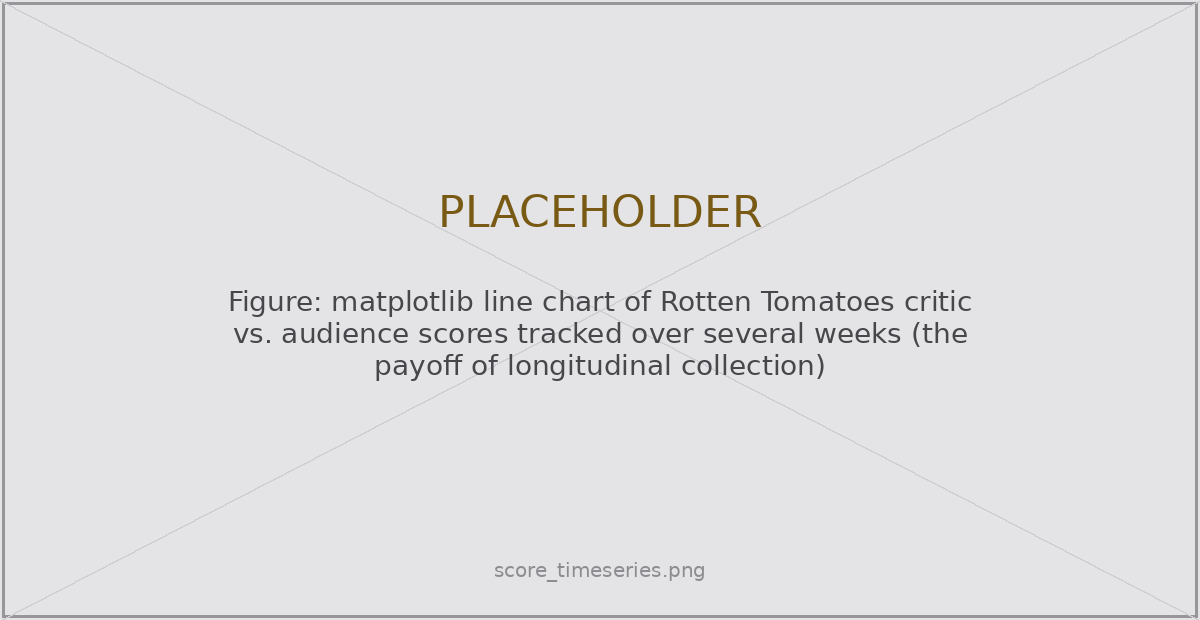
\includegraphics[width=\textwidth]{img/score_timeseries.png}\\
            {\scriptsize The payoff of collecting the same thing, repeatedly.}
        \end{column}
    \end{columns}
    \bottomcite{Textbook Ch.~14, ``Why Automate?''}
\end{frame}

\begin{frame}{Automation raises the stakes}
    \begin{columns}[T]
        \begin{column}{0.6\textwidth}
            A manual scrape you run once makes a handful of requests. A scraper running \textbf{every hour, indefinitely}, accumulates a far larger footprint --- so the ethics of Chapter~2 scale up with it.

            \vspace{0.9em}

            Automation is also how you build the \textbf{ownership} the post-API chapter describes: infrastructure that runs on \textit{your} terms and schedule, not on platform goodwill.

            \vspace{0.9em}

            But ownership is \textbf{stewardship}: monitoring, maintaining, and updating scrapers is ongoing labor. Building your own data infrastructure means accepting responsibility for its upkeep.
        \end{column}
        \begin{column}{0.36\textwidth}
            \begin{block}{Threads we pull forward}
                \footnotesize
                \begin{itemize}\footnotesize
                    \item \textbf{Ethics} --- a bigger footprint, the same politeness rules
                    \item \textbf{Protocols} --- reuse retries \& backoff for flaky runs
                    \item \textbf{Research design} --- a panel dataset you can actually analyze
                \end{itemize}
            \end{block}
        \end{column}
    \end{columns}
    \bottomcite{Textbook Ch.~14, ``Public Interest Connection.'' Post-API framing: \textcite{perriam2020digital}; \textcite{freelon2018computational}.}
\end{frame}

\begin{frame}{What the notebook builds}
    Wednesday's companion notebook builds the pipeline one step at a time:
    \begin{itemize}
        \item \textbf{Step 1} --- convert a Rotten Tomatoes scraper from a notebook into a standalone script with headless Selenium
        \item \textbf{Step 2} --- wrap it in a GitHub Actions workflow that runs every six hours
        \item \textbf{Monitor} --- catch failures and ``silent successes''; harden the workflow
        \item \textbf{Step 3} --- read the accumulated CSV back into pandas and plot the time series
    \end{itemize}

    \vspace{1em}

    \begin{alertblock}{Test locally first}
        A \texttt{print()} you can run instantly beats debugging inside YAML, where every attempt is a commit, a push, and a wait for the runner. If it runs on your machine, it will very likely run in Actions.
    \end{alertblock}
\end{frame}

% =========================================================================
\section{Wednesday · Notebook Lab}
% =========================================================================

\begin{frame}[fragile]{Step 1 --- notebook to script}
    \begin{columns}[T]
        \begin{column}{0.56\textwidth}
\begin{lstlisting}
# scraper.py -- a standalone script; no notebook
import csv, os

FIELDNAMES = ["timestamp", "url",
              "critic_score", "audience_score"]

def get_scores(url): ...   # Selenium (next slide)
def save_scores(scores): ...  # append one CSV row

def main():
    save_scores(get_scores(URL))

if __name__ == "__main__":   # the entry point
    main()
\end{lstlisting}
        \end{column}
        \begin{column}{0.42\textwidth}
            Three moves turn a notebook into production code:
            \begin{itemize}\small
                \item Wrap the work in a \texttt{main()} and guard it with \texttt{if \_\_name\_\_ == "\_\_main\_\_"} so it runs \textit{only} when executed directly.
                \item Pin the schema in \texttt{FIELDNAMES} --- a fixed column order that stays stable across every run.
                \item Open the CSV in \textbf{append} mode: each run adds one timestamped row.
            \end{itemize}
        \end{column}
    \end{columns}
    \bottomcite{Textbook Ch.~14, ``Step 1: Notebook to Script.''}
\end{frame}

\begin{frame}[fragile]{Headless Selenium on a server}
    \begin{columns}[T]
        \begin{column}{0.58\textwidth}
\begin{lstlisting}
opts = Options()
opts.add_argument("--headless")   # no window
opts.add_argument("--no-sandbox") # req'd on CI
opts.add_argument("--disable-dev-shm-usage")
driver = webdriver.Chrome(options=opts)

driver.get(url)
WebDriverWait(driver, 10).until(  # let JS render
  EC.presence_of_element_located(
    (By.TAG_NAME,
     "score-icon-critic-deprecated")))
soup = BeautifulSoup(
    driver.page_source, "html.parser")
\end{lstlisting}
        \end{column}
        \begin{column}{0.4\textwidth}
            \texttt{--headless} runs Chrome with no window; \texttt{--no-sandbox} and \texttt{--disable-dev-shm-usage} are required on a GitHub Actions runner.

            \vspace{0.6em}

            Read \texttt{page\_source} \textit{after} \texttt{WebDriverWait} --- reading a JS-heavy page too early yields empty scores.

            \vspace{0.6em}

            The \texttt{-deprecated} element names are the site's own web components; the suffix warns they change often. When they do, fix it in dev tools, not here.
        \end{column}
    \end{columns}
    \bottomcite{Textbook Ch.~14, ``Notebook to Script.'' Selenium ecosystem: \textcite{garcia_SurveySeleniumEcosystem_2020}.}
\end{frame}

\begin{frame}[fragile]{Step 2 --- schedule it with GitHub Actions}
    A YAML file in \texttt{.github/workflows/} runs your script on GitHub's cloud:
\begin{lstlisting}
# .github/workflows/scraper-action.yml
name: Scrape Rotten Tomatoes Scores
on:
  schedule:
    - cron: "0 */6 * * *"     # every 6 hours (UTC)
  workflow_dispatch:           # manual "Run workflow" button
permissions:
  contents: write              # WITHOUT this, git push fails (403)
jobs:
  scrape:
    runs-on: ubuntu-latest
    steps:
      - uses: actions/checkout@v4
      - uses: actions/setup-python@v5
        with: {python-version: "3.11"}
      - run: pip install -r requirements.txt
      - uses: browser-actions/setup-chrome@v1   # matched ChromeDriver
      - run: python scraper.py
      - run: |                                  # commit new rows
          git diff --staged --quiet || git commit -am "scores $(date -u)"
          git pull --rebase origin main && git push
\end{lstlisting}
    \bottomcite{Textbook Ch.~14, ``Step 2: GitHub Actions.'' The default \texttt{GITHUB\_TOKEN} is read-only --- \texttt{contents: write} is not optional.}
\end{frame}

\begin{frame}[fragile]{Scheduling with cron --- and a Python-free option}
    \begin{columns}[T]
        \begin{column}{0.5\textwidth}
            Five fields: \texttt{minute hour day month weekday}. All times \textbf{UTC}.
            \vspace{0.4em}

            \begin{center}\small
            \begin{tabular}{ll}
                \toprule
                Expression & Runs \\
                \midrule
                \texttt{0 */6 * * *}  & Every 6 hours \\
                \texttt{0 12 * * 1-5} & Weekdays, noon \\
                \texttt{30 8 * * *}   & Daily, 8:30 AM \\
                \texttt{0 0 1 * *}    & First of month \\
                \texttt{0 0 * * 0}    & Sundays, midnight \\
                \bottomrule
            \end{tabular}
            \end{center}
            \vspace{0.3em}
            {\footnotesize Not every scraper needs Python --- \texttt{curl} a JSON API straight from YAML:}
\begin{lstlisting}
- run: |
    D=$(date -u -d yesterday +%Y/%m/%d)
    curl -s ".../pageviews/top/en/$D" \
      -o data/top.json   # no Python
\end{lstlisting}
        \end{column}
        \begin{column}{0.46\textwidth}
            \centering
            
\includegraphics[width=\textwidth]{img/crontab_guru.png}\\
            {\scriptsize \texttt{crontab.guru} translates an expression into plain English. Bookmark it.}
        \end{column}
    \end{columns}
    \bottomcite{Textbook Ch.~14, ``Understanding Cron Syntax'' \& ``Python-Free Scraping.'' Actions may delay scheduled runs by minutes.}
\end{frame}

\begin{frame}[fragile]{Fail loudly: monitor \& harden}
    \begin{columns}[T]
        \begin{column}{0.56\textwidth}
            The insidious failure is the \textbf{silent success}: the run is green, but the CSV row is all empty --- the site changed and no exception fired. Catch it with a validation step and a graceful exit:
\begin{lstlisting}
def main():
    try:
        save_scores(get_scores(URL))
    except Exception as e:
        print(f"failed: {e}", file=sys.stderr)
        sys.exit(1)   # mark the step FAILED
\end{lstlisting}
\begin{lstlisting}
- name: Validate results     # in the workflow
  run: tail -1 scores.csv | grep -q ",," \
    && { echo "empty!"; exit 1; } || true
\end{lstlisting}
        \end{column}
        \begin{column}{0.4\textwidth}
            \centering
            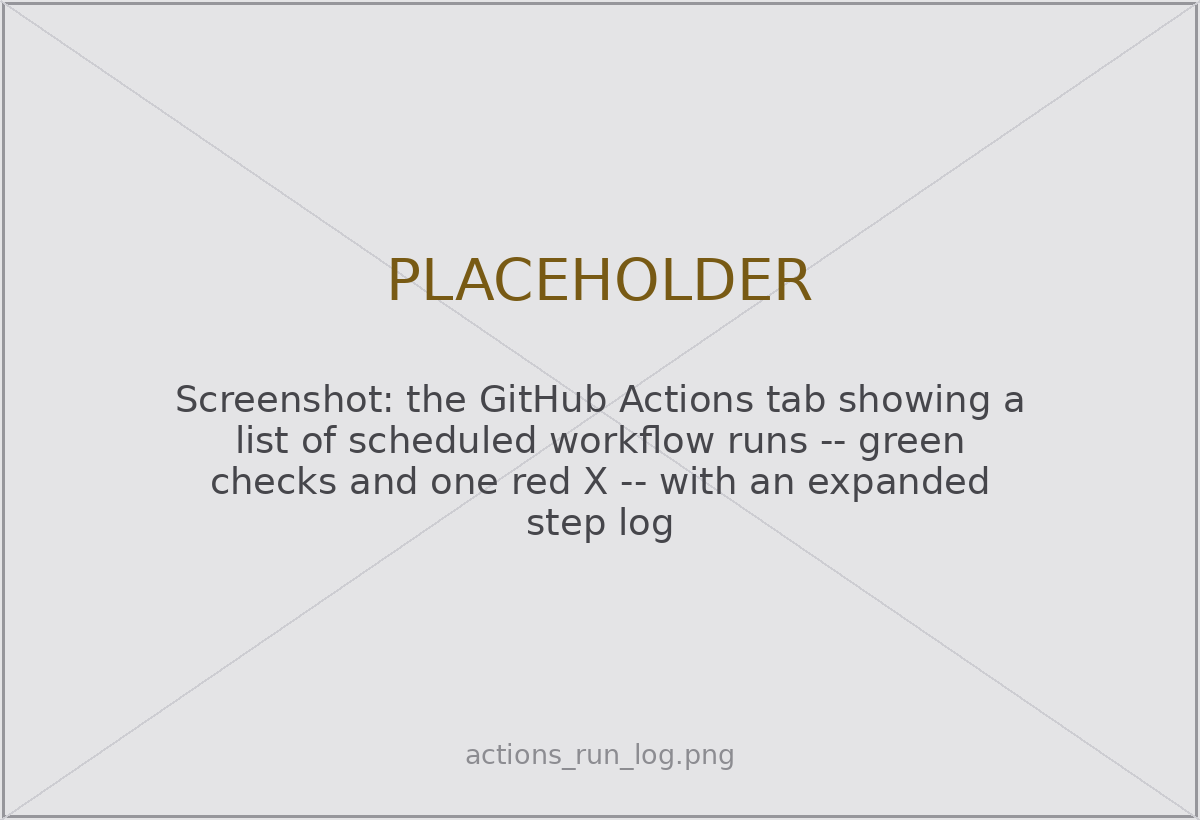
\includegraphics[width=\textwidth]{img/actions_run_log.png}\\
            {\scriptsize The Actions tab: green is not enough --- read the log.}

            \vspace{0.5em}
            {\footnotesize Harden further: \texttt{timeout-minutes} kills a hung job, a \texttt{concurrency} group stops overlaps, pip caching speeds runs, and retry-with-backoff (Ch.~Protocols) rides out transient 503s.}
        \end{column}
    \end{columns}
    \bottomcite{Textbook Ch.~14, ``Monitoring,'' ``Handling Failures,'' \& ``Hardening the Workflow.''}
\end{frame}

\begin{frame}{Lab: work these, then show-and-tell}
    \begin{columns}[T]
        \begin{column}{0.62\textwidth}
            Work through the notebook exercises in pairs:
            \begin{enumerate}\small
                \item Build \& deploy a Actions scraper; run it $\geq$3 days, then analyze
                \item Convert an earlier project to a headless \texttt{.py} script; run it from the terminal
                \item Design a monitoring check (file size, row count, or freshness)
                \item Government data (Open-Meteo, OpenAQ, USGS): collect a week, visualize the change
                \item \texttt{check\_freshness.py}: warn if the newest row is $>$24h old
                \item[6.] \textcolor{tab-purple}{\textbf{5617}}: run a collector $\geq$2 weeks, then write an infrastructure post-mortem in the spirit of \textcite{wilson2017good}
            \end{enumerate}
        \end{column}
        \begin{column}{0.34\textwidth}
            \begin{block}{Show-and-Tell}
                \footnotesize Come ready to share:
                \begin{itemize}\footnotesize
                    \item a challenging bug
                    \item interesting data you pulled
                    \item a provocation for a research design
                \end{itemize}
            \end{block}
        \end{column}
    \end{columns}
\end{frame}

\begin{frame}[standout]
    Automation is not ``set and forget.''\\
    A scraper that runs every hour, forever,\\
    is a promise you make to maintain it.\\[1em]
    {\large Ownership is stewardship.}
\end{frame}

% =========================================================================
\section{Friday · Textbook Revisions}
% =========================================================================

\begin{frame}{Improving Chapter 14 together}
    \begin{columns}[T]
        \begin{column}{0.6\textwidth}
            Today we make the book better. Each of you opens a \textbf{pull request} against \texttt{ch-14-automation.qmd} and reviews a classmate's.

            \vspace{1em}

            The workflow (from Week 1):
            \begin{enumerate}\small
                \item Branch / fork the book repo
                \item Edit the chapter; commit with a clear message
                \item Open a PR describing \textit{what} and \textit{why}
                \item Review two peers' PRs: kind, specific, actionable
            \end{enumerate}
        \end{column}
        \begin{column}{0.36\textwidth}
            \centering
            
\includegraphics[width=\textwidth]{img/pr_review.png}
        \end{column}
    \end{columns}
    \bottomcite{Contributions \& reviews count toward the Textbook Revisions grade (30\%).}
\end{frame}

\begin{frame}{A revision menu for Chapter 14}
    High-value targets --- pick one and scope it to a single PR:
    \begin{itemize}
        \item \textbf{Run the workflow live.} Fork the repo, trigger the Action, and report what broke --- selector drift on the \texttt{-deprecated} elements, or a ChromeDriver mismatch. Document the fix (this is the chapter's own fragility warning).
        \item \textbf{Deepen ``Common Issues to Debug.''} Add a worked YAML-indentation failure, a \texttt{git pull --rebase} conflict walkthrough, or a \texttt{webdriver-manager} recipe for local driver drift.
        \item \textbf{Add a figure.} An annotated Actions run-log screenshot, the notebook$\rightarrow$script$\rightarrow$pipeline diagram, or a \texttt{crontab.guru} capture would each help.
        \item \textbf{Make an exercise turnkey.} Ship a starter \texttt{requirements.txt} + workflow template and expected output so Exercises 1 and 4 are self-checking.
        \item \textbf{Extend ``Further Reading.''} A public-interest collector (air-quality network, transit tracker) tied to the ownership callout.
    \end{itemize}
    \bottomcite{Targets drawn from the chapter's callouts, ``Common Issues,'' and ``Further Reading.''}
\end{frame}

\begin{frame}{What makes a good revision \& a good review}
    \begin{columns}[T]
        \begin{column}{0.48\textwidth}
            \begin{block}{A strong PR}
                \begin{itemize}\small
                    \item One focused change, clearly titled
                    \item Explains the problem it fixes
                    \item Builds (\texttt{quarto render}) without errors
                    \item Matches the book's voice and notation
                    \item Discloses any AI assistance
                \end{itemize}
            \end{block}
        \end{column}
        \begin{column}{0.48\textwidth}
            \begin{block}{A strong review}
                \begin{itemize}\small
                    \item Runs / reads the change, not just skims
                    \item Names specifics (line, claim, code)
                    \item Separates ``must fix'' from ``nice to have''
                    \item Is generous --- assume good faith
                    \item Ends with a clear verdict
                \end{itemize}
            \end{block}
        \end{column}
    \end{columns}
    \vspace{0.5em}
    \centering\small Next week: \textbf{research design} --- turning your automated collection into an end-to-end project.
\end{frame}

% =========================================================================
\begin{frame}{Key takeaways}
    \begin{enumerate}
        \item Production collection is a progression: \textbf{notebook $\rightarrow$ script $\rightarrow$ scheduled pipeline} --- the same code, moved into production.
        \item Run once for a \textbf{snapshot}; run on a schedule for a \textbf{time series} (a panel dataset you can actually analyze).
        \item GitHub Actions gives free cloud scheduling; set \texttt{permissions: contents: write} or \texttt{git push} 403s, and remember cron is \textbf{UTC}.
        \item \textbf{Fail loudly}: validate output to catch silent successes, wrap scrapes in try/except, and harden with timeouts, concurrency, and backoff.
        \item Automation is not ``set and forget'' --- owning your data infrastructure means committing to its \textbf{stewardship}.
    \end{enumerate}
    \vspace{1em}
    \bottomcite{Reading: Textbook Ch.~14. Related: \textcite{munzert2014automated}; \textcite{mitchell2018web}. Archival precedents: \textcite{baumgartner2020pushshift}.}
\end{frame}

\end{document}
